% Chapter 2: 相关理论及技术 (Related Theory and Technology)
\chapter{相关理论及技术}

为了给后续各章的算法改进与应用验证提供坚实的理论支撑，本章将系统梳理研究所涉及的核心技术与理论框架。内容涵盖了元启发式搜索机制、复杂优化任务的数学建模、代理辅助优化策略，以及用于性能评估的统计分析方法。

\section{元启发式优化算法}

元启发式算法（MAs）已成为现代复杂优化领域的重要方法论基础，尤其在处理搜索空间庞大且缺乏显式解结构的NP-hard问题时，表现出显著的灵活性和鲁棒性\cite{ibsa_ref4,sbo_ref1}。这些方法按其灵感来源的多样性，通常被划分为群体智能、进化计算、自然规律模拟以及人类行为模仿等不同体系\cite{sbo_ref11}。尽管不同算法的更新机制各异，但其核心目标都在于协调探索（Exploration）与开发（Exploitation），即在扩大搜索范围和强化局部精炼之间取得平衡\cite{ibsa_ref75}。

\subsection{群体智能与进化算法}

群体智能算法通过个体间的信息共享与协同更新实现全局搜索\cite{sbo_ref18}。粒子群优化（PSO）\cite{ibsa_ref26}是其中最具代表性的方法之一，其基本更新规则为：
\begin{equation}
v_i^{t+1} = \omega v_i^t + c_1 r_1 (pbest_i - x_i^t) + c_2 r_2 (gbest - x_i^t)
\end{equation}
\begin{equation}
x_i^{t+1} = x_i^t + v_i^{t+1}
\end{equation}
其中，$\omega$为惯性权重，$c_1$和$c_2$为学习因子，$r_1$和$r_2$为$[0,1]$上的随机数，$pbest_i$和$gbest$分别表示个体历史最优位置与群体全局最优位置。PSO因概念简洁和实现高效，已被广泛应用于函数优化、神经网络训练和组合优化等领域。除PSO外，灰狼优化算法（GWO）\cite{ibsa_ref81}通过模拟灰狼的社会等级和狩猎行为实现群体搜索，蚁群优化算法（ACO）\cite{ibsa_ref25}借鉴蚂蚁信息素沉积机制解决离散优化问题，人工蜂群算法（ABC）\cite{ibsa_ref27}模拟蜜蜂觅食行为进行全局搜索。这些算法各有特色，共同构成了群体智能优化方法的基本框架。

与模拟群体行为不同，进化算法更侧重于遗传变异规律的工程模拟\cite{sbo_ref11}。差分进化（DE）\cite{ibsa_ref34}结构简洁，在实值优化任务中收敛稳定，已成为代理辅助优化中的常用搜索工具。常用的DE/rand/1变异策略通过向量间的差分驱动搜索：
\begin{equation}
v_i = x_{r1} + F \cdot (x_{r2} - x_{r3})
\end{equation}
其中，缩放因子$F$与交叉概率$CR$共同调控了变异幅度和个体多样性。这种贪心驱动的迭代机制不仅保证了收敛的稳定性\cite{ibsa_ref55}，也为后续各章的算法设计提供了基本的种群演化框架。

\subsection{回溯搜索算法}

回溯搜索算法（BSA）由Civicioglu\cite{ibsa_ref53}于2013年提出，是一种利用历史种群记忆进行搜索的进化算法。其主要流程包括初始化、Selection-I、变异、交叉和Selection-II五个阶段，其中变异策略利用当前种群与历史种群之间的差异生成候选解：
\begin{equation}
\boldsymbol{Mutant} = \boldsymbol{X} + F \cdot (\boldsymbol{OldX} - \boldsymbol{X})
\end{equation}
其中，$F = 3 \cdot rndn$。历史记忆策略提升了全局探索的潜力，但由于变异与交叉逻辑带有较强的随机性，在局部精细化搜索方面仍有不足\cite{ibsa_ref63}。Zhao\cite{ibsa_ref57}与Nama\cite{ibsa_ref59}等学者提出的策略改进方案，直接启发了本文在第三章中对IBSA算法的设计思路。

\subsection{探索与开发平衡性}
\label{sec:ch2_balance_diversity}

为定量分析算法在搜索过程中的动态行为，本研究引入基于种群多样性的度量指标。维度多样性$\text{Div}(t)$定义为：
\begin{equation}
\text{Div}(t)=\frac{1}{D}\sum^D_{j=1}{\frac{1}{N}\sum^N_{i=1}{\left|\operatorname{median}\left(X^j\left(t\right)\right)-X^j_i\left(t\right)\right|}}
\end{equation}

在此基础上，探索率与开发率分别定义为：
\begin{equation}
\text{Exploration}=\frac{\text{Div}\left(t\right)}{\text{Div}_{\max}}\times 100\%
\end{equation}
\begin{equation}
\text{Exploitation}=\frac{\left|\text{Div}\left(t\right)-\text{Div}_{\max}\right|}{\text{Div}_{\max}}\times 100\%
\end{equation}
进一步地，基于种群质心的欧氏距离多样性$I_C(t)$为：
\begin{equation}
I_C(t) = \sqrt{\sum^{N}_{i=1}{\sum^{D}_{j=1}{{\left(X^j_i\left(t\right)-C^j(t)\right)}^{2}}}}
\end{equation}
\begin{equation}
C^j(t) = \frac{1}{N}\sum^N_{i=1}{X^j_i\left(t\right)}
\end{equation}
$I_C(t)$越大，种群整体分散程度越高，说明算法处于探索阶段；$I_C(t)$较小时种群趋于聚集，算法处于开发阶段。较理想的优化过程应在搜索前期保持较高的多样性，并在后期逐步收缩以精炼最优解。第三章和第四章将利用这些指标分析所提算法的搜索特性。

\section{特征选择与图像分割问题简介}

本研究所涉及的两个主要应用场景——高维特征筛选与医学影像分割，本质上均是对候选参数的寻优过程。前者需要在离散组合空间中搜索最优特征子集，后者则是在连续或准离散的灰度阈值空间中寻找最优分割参数。

\subsection{特征选择问题定义}

特征选择（FS）旨在从原始特征中筛选出对任务贡献最大的子集，在保持或提升模型性能的同时降低维度，缓解维数灾难并增强可解释性\cite{ibsa_ref50}。常见方法包括过滤式、嵌入式和包裹式三类\cite{sbo_ref61}：过滤式依赖统计指标进行独立筛选，计算效率高但难以刻画特征交互\cite{sbo_ref62}；嵌入式将特征选择融入模型训练过程；包裹式直接以分类器性能评价特征子集，效果通常更好，但计算成本较高\cite{ibsa_ref23,sbo_ref64}。

在基于元启发式的包裹式特征选择中，每个特征对应一个0/1决策变量，问题可视为二值优化。由于多数元启发式算法面向连续空间，通常需借助V型传递函数完成二值化：
\begin{equation}
T(x) = \left| \operatorname{erf}\left(\frac{\sqrt{\pi}}{2} x\right) \right|
\end{equation}
若$T(x_i^d) > rand$，则对应维度取值翻转，否则保持不变。为同时兼顾分类误差和特征压缩率，适应度函数定义为：
\begin{equation}
\text{Fitness}=\alpha\cdot \gamma_R\left(N\right)+\beta\cdot \frac{\left|R\right|}{\left|N\right|}
\end{equation}
后续实验将从平均适应度、分类错误率、选择特征数和运行时间四个方面评估算法表现。

\subsection{多阈值图像分割问题}

多阈值图像分割通过确定多个阈值将图像灰度空间划分为若干区域，是医学图像分析中的常见预处理步骤\cite{sbo_ref79,sbo_ref80}。若图像灰度级为$L$，阈值向量可表示为：
\begin{equation}
\boldsymbol{T} = [t_1, t_2, \ldots, t_K], \quad 0 \le t_1 < t_2 < \cdots < t_K \le L-1
\end{equation}
其中$K$为阈值个数。随着$K$增加，候选解空间迅速膨胀，传统穷举方法难以在可接受时间内获得满意解。利用元启发式算法在这类大规模搜索空间中高效搜索最优阈值组合，已成为该领域的主流做法\cite{sbo_ref82}。本文第四章采用Renyi熵评价阈值集合质量，并利用元启发式算法搜索最优阈值，以提高乳腺癌组织学图像\cite{sbo_ref83}的分割效果。

\section{代理辅助昂贵优化技术}

在昂贵优化问题（EOPs）中，单次目标函数评估通常依赖高保真仿真或复杂工程计算，代价极高\cite{liu2023airfoils,kumar2024optimization}。代理辅助进化算法（SAEAs）通过低成本模型近似真实目标函数，以减少真实评估次数\cite{he2023review,jin2018data}，是第五章方法设计的理论基础。

\subsection{代理模型与填充准则}
\label{sec:ch2_surrogate_models}

代理模型用于学习真实目标函数的近似映射\cite{kudela2022recent}。径向基函数（RBF）模型是一种基于距离的插值方法\cite{regis2013evolutionary}，其预测值为已知样本点处基函数的加权组合：
\begin{equation}
\hat{f}(x) = \sum_{i=1}^{n} \lambda_i \phi(\|x - x_i\|)
\end{equation}
由插值条件$\hat{f}(x_i) = f(x_i)$可得矩阵形式：
\begin{equation}
\mathcal{F} = \boldsymbol{\Psi} \mathcal{W}
\end{equation}
其中$\boldsymbol{\Psi}_{ij} = \phi(\|x_i - x_j\|)$。RBF模型训练速度快、插值精度高，对高维问题适应性较好\cite{kudela2022recent}，因此在第五章中被选作基础代理模型。

图\ref{fig:ch2_RBF_prediction}展示了利用六个均匀分布样本对一维函数进行RBF近似的结果\cite{forrester2008engineering}。白色圆圈表示样本点，黑色实线代表真实适应度景观，红色虚线代表RBF预测函数。从图中可以看出，RBF模型在样本点处能够精确插值，而在样本点之间给出平滑近似。

\begin{figure}[!b]
    \centering
    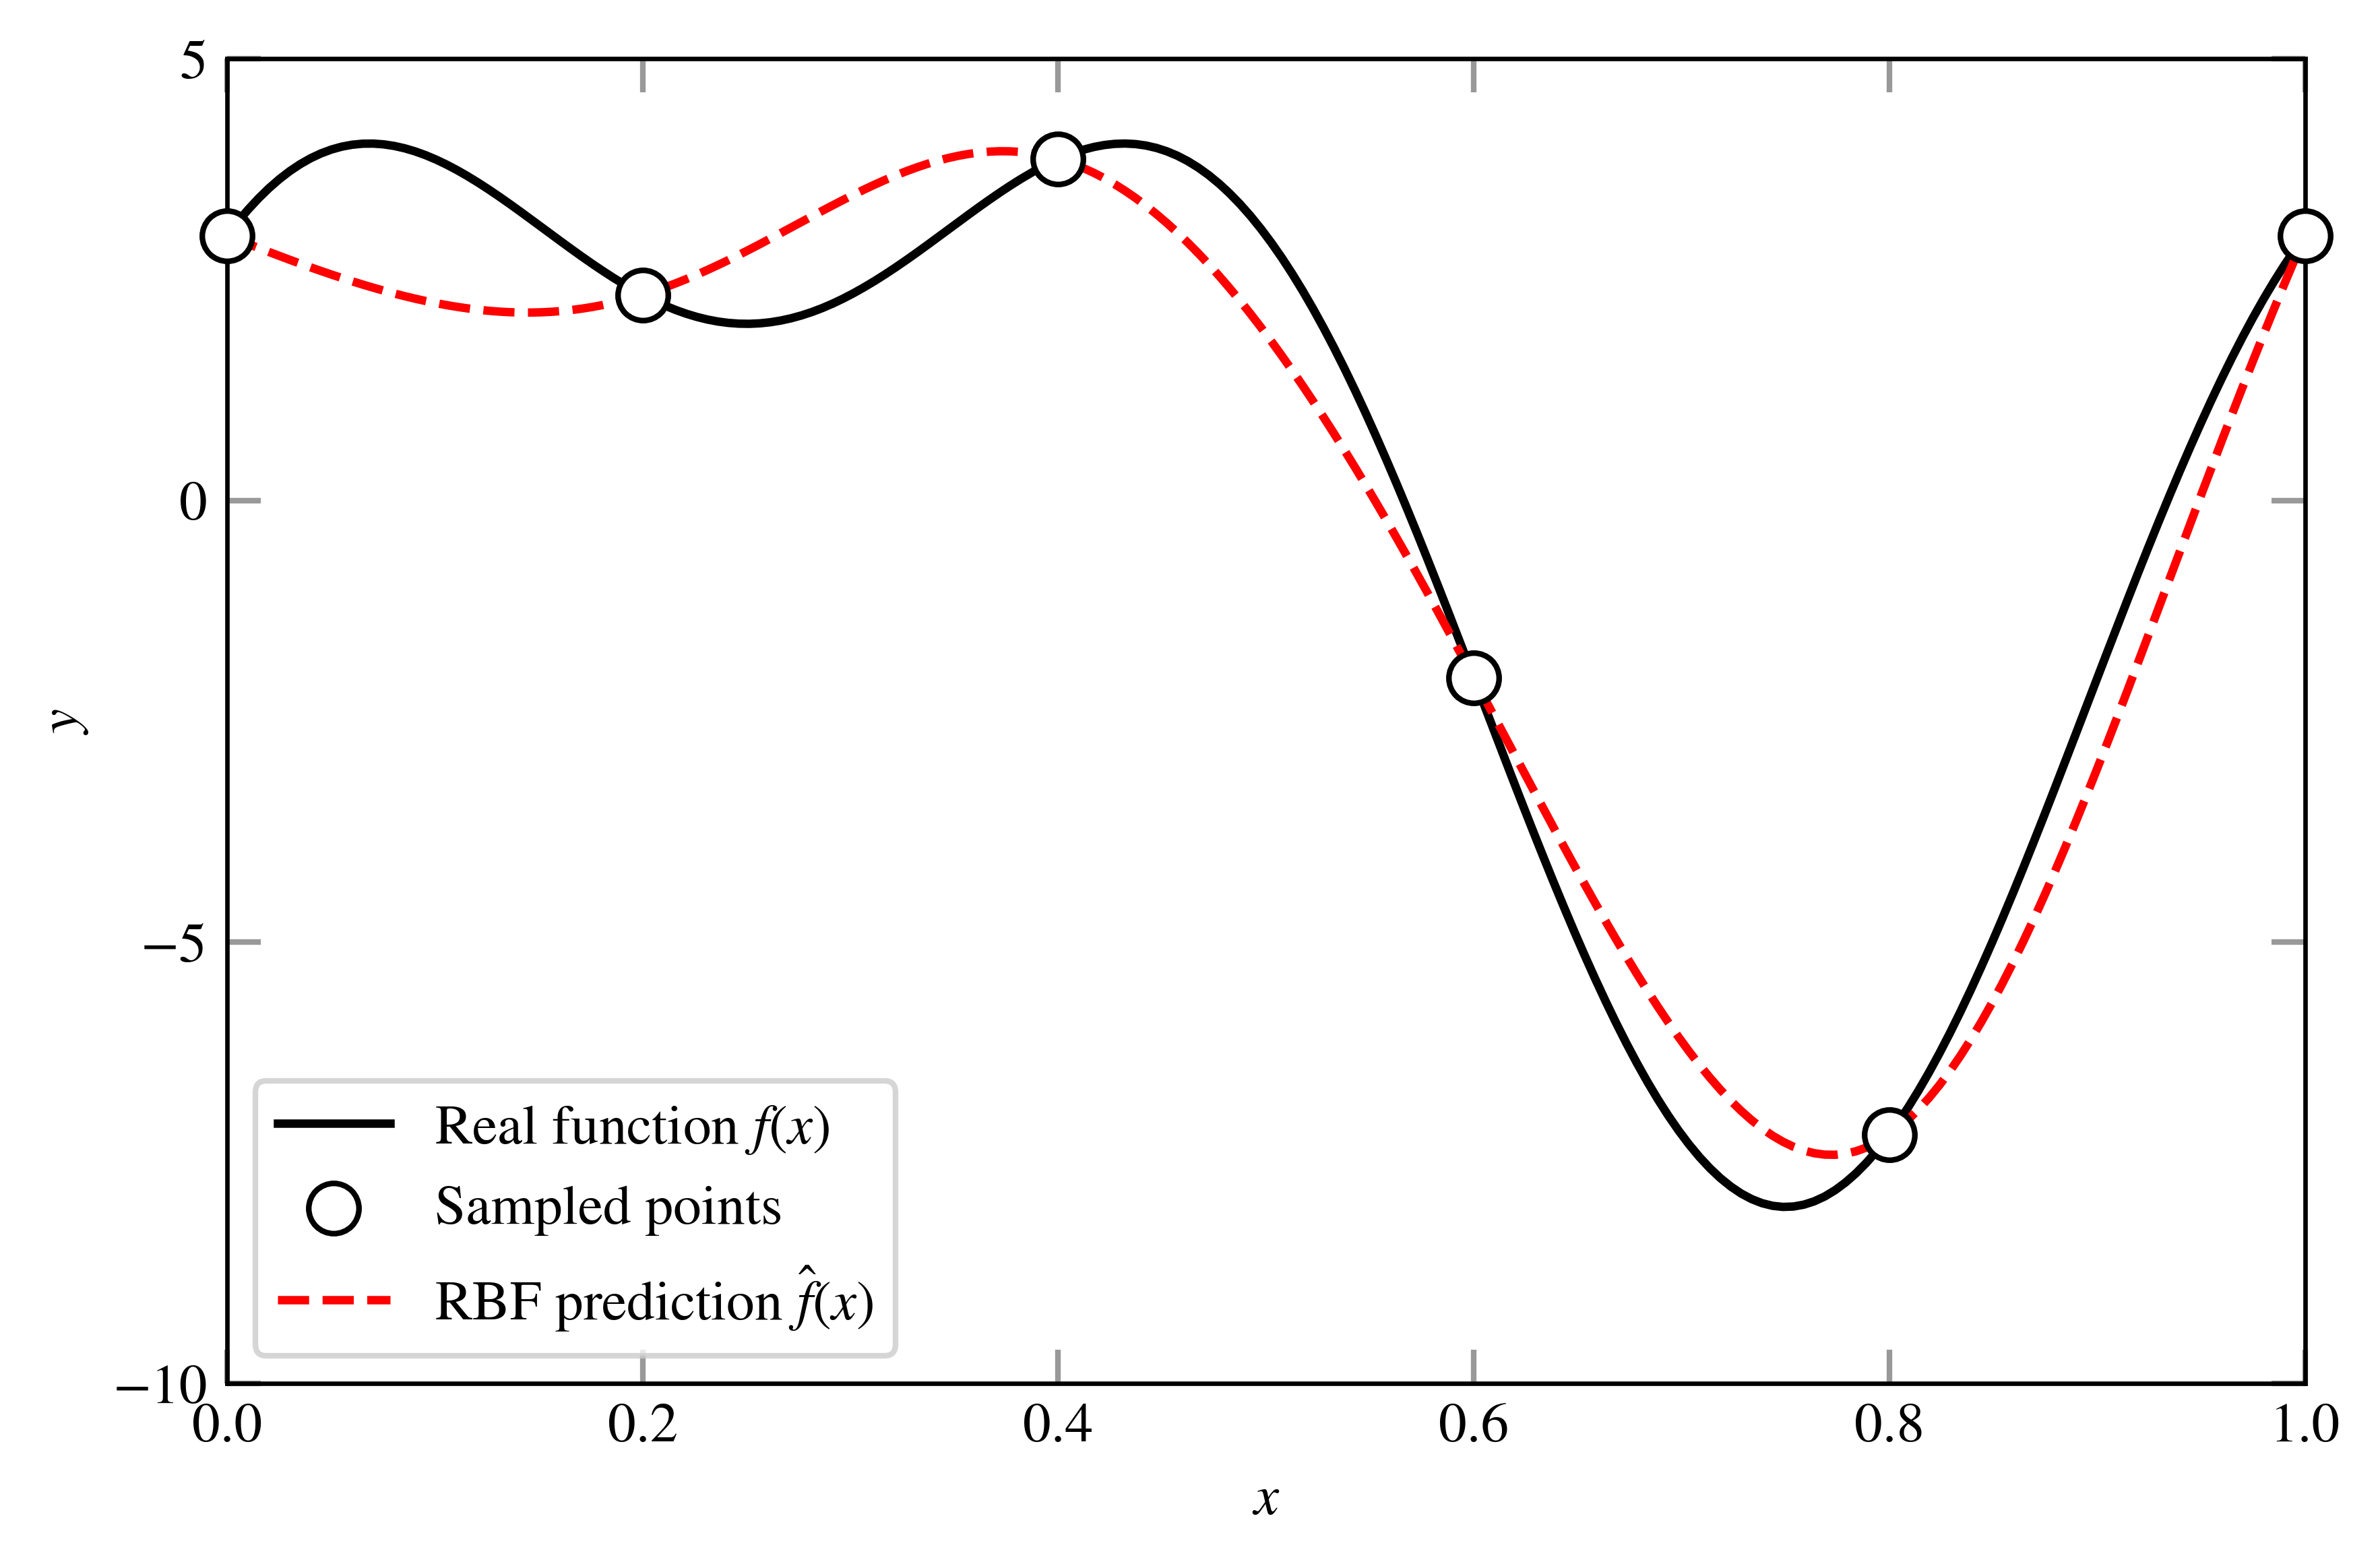
\includegraphics[width=0.92\linewidth]{figures/chapter5/rbf_plot.png}
    \bicaption{一维函数上的RBF预测}{RBF prediction on a 1-dimensional function}
    \label{fig:ch2_RBF_prediction}
\end{figure}

Kriging模型（高斯过程模型）\cite{buche2005accelerating,liu2013gaussian}除给出预测值外，还能提供不确定性估计，因此常与采样决策联合使用。为从候选解中筛选最值得进行真实评估的样本，通常需要引入填充准则\cite{zhan2020expected}。期望改进（EI）\cite{jones1998efficient}定义为：
\begin{equation}
EI(x) = (f_{min} - \hat{f}(x)) \Phi\left(\frac{f_{min} - \hat{f}(x)}{s(x)}\right) + s(x) \phi\left(\frac{f_{min} - \hat{f}(x)}{s(x)}\right)
\end{equation}
其中，$f_{min}$为当前最优值，$\hat{f}(x)$和$s(x)$分别为代理模型的预测均值和标准差，$\Phi$和$\phi$分别为标准正态分布的累积分布函数和概率密度函数。置信下界（LCB）则定义为：
\begin{equation}
LCB(x) = \hat{f}(x) - \kappa \cdot s(x)
\end{equation}
其中，$\kappa$越大则越倾向于探索。EI和LCB都体现了对探索与开发的联合考虑，使代理辅助优化能够在有限评估预算下做出较合理的采样决策。

\subsection{多臂赌博机策略}

多臂赌博机（MAB）问题描述了决策者如何在多个候选动作之间权衡已知高收益选择与未知选择\cite{slivkins2019introduction}，其核心是探索与开发的平衡。在优化算法中，可将不同搜索算子视为不同臂，根据环境反馈自适应地调整选择概率\cite{xie2023surrogate,gong2024surrogate}。

上置信界（UCB）策略是解决MAB问题的经典方法之一\cite{auer2002finite}，其在第$t$轮选择具有最高上置信界的臂：
\begin{equation}
a_t = \argmax_{a} \left[ Q_t(a) + c \sqrt{\frac{\ln t}{N_t(a)}} \right]
\end{equation}
其中，$Q_t(a)$为臂$a$的估计收益均值，$N_t(a)$为臂$a$被选择的次数，$c$为探索系数。UCB策略的核心在于：$Q_t(a)$鼓励选择历史表现较好的臂（利用），探索项$c \sqrt{\ln t / N_t(a)}$则鼓励尝试被选次数较少的臂（探索），随着总选择次数增长，探索项逐步衰减，策略自然收敛到最优臂。第五章将在此基础上引入赌博机驱动的自适应搜索机制，将不同搜索模式建模为不同臂，根据实时优化反馈动态切换搜索策略。

\section{基准测试与统计检验}

\subsection{基准测试函数}

基准测试函数为算法性能评估提供了统一且可复现的比较环境\cite{ibsa_ref4}。IEEE CEC 2017测试套件包含30个函数，覆盖单峰（F1--F3）、多峰（F4--F10）、混合（F11--F20）和组合（F21--F30）四类问题\cite{ibsa_ref88}，能够全面考察算法在不同搜索景观下的表现，本文第三章和第四章均采用该测试套件。IEEE CEC 2022测试套件面向函数评估受限的昂贵优化场景，包含12个函数\cite{kumar2024optimization}，最大评估次数受到严格限制，本文第五章使用其评估BEXEA的性能。

\subsection{统计检验方法}
\label{sec:ch2_stat_tests}

为保证实验比较的统计有效性，本文采用非参数统计检验对算法结果进行严格分析。Wilcoxon秩和检验\cite{ibsa_ref95}是一种成对比较方法，通过对两组独立样本的排名差异进行分析，判断二者是否具有统计显著性差异，适合样本量较小或数据不满足正态分布假设的情况。Friedman检验\cite{derrac2011practical}则是一种多组比较方法，可同时对多个算法在多个测试函数上的排名进行整体比较，排名越低表示综合表现越好。后续各章中，符号"+"、"="和"-"分别表示所提算法在Wilcoxon检验中显著更优、结果相当和显著更差，显著性水平设为$\alpha=0.05$。

\section{本章小结}

本章围绕后续研究的共性需求，对元启发式优化算法、特征选择与图像分割问题、代理辅助昂贵优化技术以及基准测试与统计检验方法进行了概述。这些内容为第三章至第五章的算法设计、应用建模和实验分析提供了统一的理论基础。




